\chapter{Bigtable}

\paragraph{Systems used} Processing with Sawzall and MapReduce
\begin{itemize}
\item Scheduler (Google WorkQueue): (failure detection, membership)?
\item GFS: Master (metadata) \& Chunk servers: (read and writing large chunks of
  data)
\item Chubby: Coarse-grained locks with small amount of data in a lock. 5 nodes
  Paxos
\end{itemize}

\paragraph{Data model} Distributed map: Atomic read or write in a single row key
\begin{itemize}
\item \texttt{<Row, Column, Timestamp>}, value is uninterpreted byte array
\item \texttt{ColumnFamily:qualifier}: Same CF $=$ Same AC \& Same compression
\item API: Lookup, insert, delete (+scan)
\item Settings: In memory SSTs, data lexicographically sorted (locality
  control)
\end{itemize}

\paragraph{SSTable}  Immutable, sorted file of key-value pairs arranged in
blocks. Index of block ranges for single disk seek. Can be shared by multiple
tablets (split).

\paragraph{Tablets} Non overlapping range of rows of a table (multiple
SSTables). Unit of distribution \& load balancing of each table. Client caches
location of tablet. Tablet history found in METADATA table.

\begin{figure}[h]
  \centering
  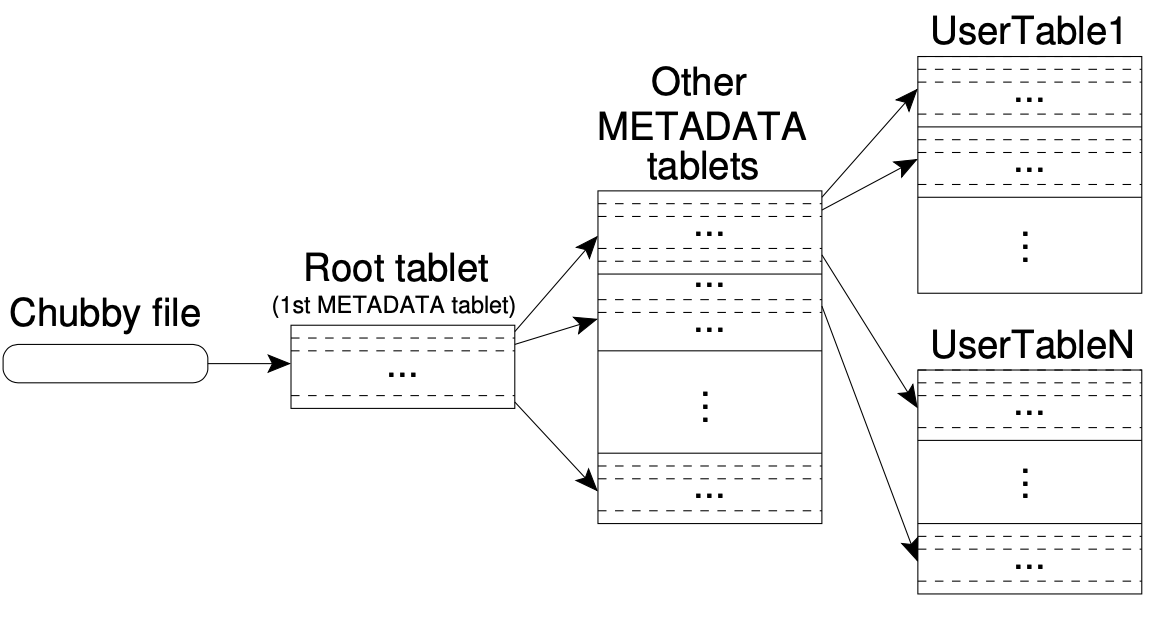
\includegraphics[width=0.4\linewidth]{img/bt-location.png}
\end{figure}

\paragraph{Server} Each tablet lives at only one server. Master assigns multiple
tablets per server, and monitors load and server fault (chubby lock). Tablet
server splits tablets that get too big. Shared server-wide commit log \& group
commit.

\paragraph{Editing/Reading a Table} Writes go in GFS REDO commit log, then
applied to (sorted) memtable (COW rows for concurrency). Reads applied to merged
view of SSTables \& memtable. R\&W continue during tablet split or merge. RPC is
checksumed and authorization happens on tablet server.

\paragraph{Compaction}
\begin{itemize}
\item \textbf{Minor compaction}: Memtable into an SSTable (Reduce memory usage,
  Reduce log traffic on restart).
\item \textbf{Major compaction}: Merging SSTables to one SSTable (No deletion
  records, only live data)
\item \textbf{Merging compaction}: Reduce number of SSTables (+policy “keep only
  N versions”)
\end{itemize}

\paragraph{Locality groups}. Group CFs into SSTables under shared compression
scheme. Can use bloom filters to avoid fetching SSTables.

\begin{figure}[h]
  \centering
  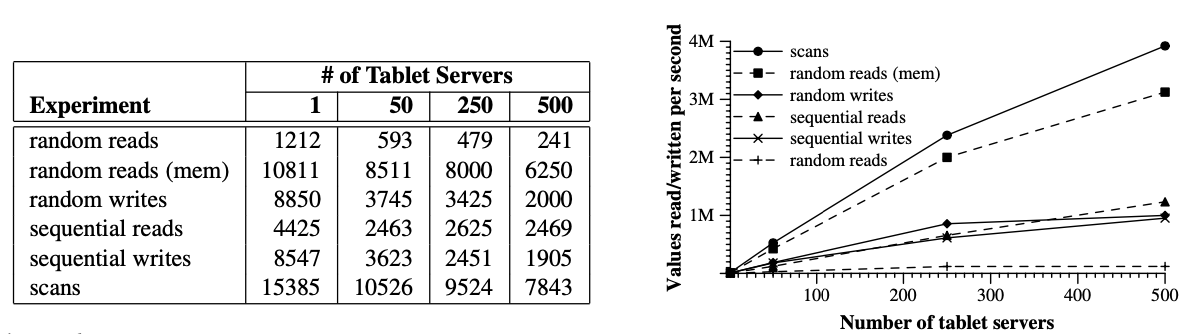
\includegraphics[width=0.95\linewidth]{img/bt-bench.png}
\end{figure}